\documentclass{article}

\title{Economic complexity and information choice}
\author{Cameron Pfiffer}

\usepackage{palatino}
\usepackage{amsmath}
\usepackage{todonotes}
\usepackage{optidef}
\usepackage{color,soul}
\usepackage{physics}
\usepackage{graphicx}
\usepackage{caption}
\usepackage{subcaption}
% \setlength{\parindent}{0pt}

\hfuzz=20pt 

\if@todonotes@disabled
    \newcommand{\hlfix}[2]{#1}
    \else
    \newcommand{\hlfix}[2]{\texthl{#1}\todo{#2}}
\fi

\usepackage[style=apa, 
backend=biber, 
giveninits=true,
uniquelist=false, 
uniquename=init,
isbn=false, 
maxcitenames=2,
dashed=false, 
maxbibnames=999,
doi=false,
url=false]{biblatex}
\addbibresource{bibs/library.bib}

\begin{document}

% Shortcut variables
\newcommand{\Gauss}{\mathcal{N}}
\newcommand{\Var}{\text{Var}}
\newcommand{\E}{\text{E}}
\newcommand{\argmax}{\text{argmax}}

% Theorem styles
\newtheorem{definition}{Definition}


\newpage

\maketitle

\section{Introduction}

A strand of economic literature studies how limited attention and cognitive constraints guide economic choices. In these papers, researchers examine how prices can be used to aggregate private signals observed by attention-constrained investors. 

The general conclusion of these papers, such as \textcite{kacperczyk_rational_2016} or \textcite{peng_investor_2006}, is that investors will rationally allocate more attention to a common component of variation in payoffs as the variance of that common component rises. A shortcoming in these papers is that the economies are extraordinarily simplistic and may understate how dramatic the effect of information choice can be when investors are confronted with complex economic environments.

Consider the example of two firms and their stocks. Company A is a domestic utility company. It has stable cashflows and is generally resistant to the business cycle. Company B is a riskier global trade venture which has state-contingent payoffs. In the good state, a foreign firm's economy experiences a boom, increasing Firm B's performance significantly. Firm B's payoffs are higher in the good state and may have different payoff variance. In the bad state, the foreign economy goes into recession, and Firm B has significantly lower payoffs with an arbitrarily different payoff variance. Assume that Firm A's payoff distribution varies only slightly between these two states, due to the small effects on domestic and international consumption that could lightly tilt the firm's performance. Investors are unable to accurately perceive the state of the foreign economy in a timely manner and must infer the state from signals about payoffs for Firms A \& B.

If an investor who wishes to forecast asset performance can only allocate a finite amount of attention between these two firms, which firm should they choose? If the investor allocates most of their attention to Firm A, they will receive a large and potentially precise signal about Firm A's payoffs but at the cost of little to no information about whether the economy is likely to be in the good state or the bad state. The question is a non-trivial one to answer, as investors make an ex-ante decision about which firms to assess, and then must choose some portfolio after observing information about each firm.

The information and portfolio choice problems essentially reduce to a single question: how useful is knowledge about the state? First, the usefulness of state knowledge depends on the choices of other investors. Prices can be used to infer the information sets of other investors (\textcite{grossman_existence_1977}). Second, the usefulness of state information depends critically on how different the states are in their conditional densities. If the good state and bad state are extremely different, it may pay for an investor to be asymmetrically informed about state even if they are less informed about specific payoffs.

I examine how endogenous information choice with attention limitations can lead investors to choose distinct portfolios when signals inform investors about both the underlying economic state and asset payoffs in those states. Allowing risk averse investors to select signals that are informative about state and payoffs jointly produces \hl{substantially different} \todo[noline]{Check if this actually happened} portfolios from standard noisy rational equilibrium models, as well as shifting the conclusions of canonical models of information choice where signals inform investors \textit{only} about payoffs.

\todo{lit review here}

\section{Model framework}

Much of my notation and model structure follows from \textcite{kacperczyk_rational_2016},  which introduce attention constraints and information choice to the multiasset noisy rational equilibrium model of \textcite{admati_noisy_1985}.

The model has three periods. In time 1, informed investors allocate their attention across $n$ signals. At time 2, all investors construct portfolios. At time 3, all investors receive payoffs.

I assume, as in \textcite{kacperczyk_rational_2016}, that there are $n$ risky assets with an arbitrary factor structure given by principal components. Assets $1,2,\dots,n$ represent specific assets with idiosyncratic shocks. The key difference between my paper and \textcite{kacperczyk_rational_2016} is that the economic state is a stochastic variable that is not known by investors. The economy is in state $s \in {H, L}$, where $s=H$ represents a "good" state with probability $\pi$ and $s=L$ represents a "bad" state with probability $1-\pi$. The density of $s$ is written

$$
P(s) = \begin{cases}
    \pi & \text{ if } s = H \\
    1-\pi & \text{ if } s = L \\
\end{cases}
$$

The good and bad states dictate the mean and covariance of asset payoffs. Payoffs of the $n$ assets, denoted by $n\times 1$ vector $f$, are written

\begin{align}
    f_i &= \mu_{i,s} + z_i\\
    z &= [z_1,z_2, \dots, z_n]' \sim \Gauss(0, \Sigma_s) \\
    f &\mid s \sim \Gauss(\mu_{s}, \Sigma_s)
\end{align}

The mean payoff vector $\mu_s = [\mu_{1,s},\mu_{2,s},\dots,\mu_{n,s}]'$ and the  $n\times n$ variance-covariance matrix of payoff shocks $\Sigma_s$ are functions of the unobserved economic state. When investors are allowed to receive signals about the underlying shocks $z$, those same signals will allow investors to assign a probability to the underlying state and the associated payoff structure.\footnote{\textcite{kacperczyk_rational_2016} utilize a transformation of asset payoffs to the corresponding risk factor payoffs -- in my case, the eigen-decomposition $\Sigma_s = \Gamma_s \Lambda_s \Gamma_s'$ for $s \in {H,L}$ yields Arrow-Debreu synthetic securities on risk factors:

\begin{align}
    \tilde f \mid s \sim \Gauss(\Gamma_s^{-1} \mu_s, \Lambda_s)
\end{align}

\noindent Unfortunately, I cannot proceed with the \textcite{kacperczyk_rational_2016} solution method, which requires an additional transformation of risk factor prices $\tilde p = \Gamma^{-1}p$ and risk factor quantities $\tilde q = \Gamma^{-1} q$ for some eigenvector matrix $\Gamma$. My model only permits the orthogonalization of the prior variance $\Sigma$, but in general the transforms on $\tilde q$ and $\tilde p$ will remain correlated conditional on state.


}

Note that the unconditional payoff density $P(f)$ is a two-component Gaussian mixture distribution with mixture weights $\pi$ and $1-\pi$. The density function is written

\begin{align}
    P(f) \sim \pi \Gauss(f \mid \mu_H, \Sigma_H) + (1-\pi) \Gauss (f \mid \mu_L, \Sigma_L)
\end{align}

\noindent Gaussian mixture distributions have the conceptual benefit of moving payoffs outside the traditional exponential family of distributions. In principle, a mixture model can approximate any complex joint density as the number of components increase (\cite{nguyen_approximations_2019}). I maintain only two components as a proof-of-concept, though much of my analysis expands easily to an arbitrary number of Gaussian components. Additionally, many of the posterior distributions are only marginally more complex than when using traditional normal or log-normal distributions.

% \begin{figure}
%     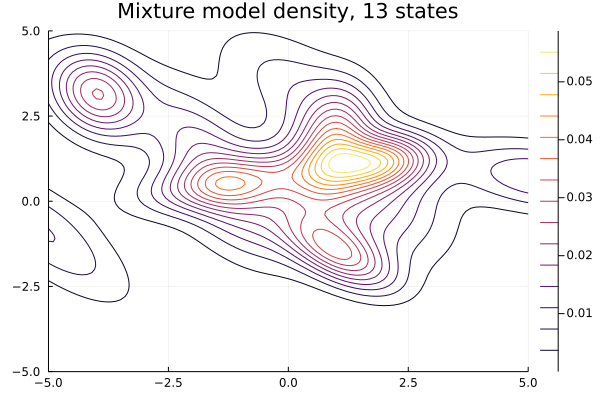
\includegraphics[width=\textwidth,height=\textheight,keepaspectratio]{plots/mixture-1.png}
%     \caption{The joint density contour plot of a multimodal Gaussian mixture distribution. Dimensionality is $\mathcal{R}^2$.}
% \end{figure}

As in \textcite{admati_noisy_1985} and \textcite{kacperczyk_rational_2016}, I employ CARA utility to abstract from wealth effects. However, the conditions in \textcite{kacperczyk_rational_2016} that reduce the investment problem to a mean-variance problem do not hold in my setting without minor modifications. Namely, the distribution of $f$ is unconditionally non-Gaussian. Fortunately, the Gaussian mixture distribution I pay off benefits from the fact that the non-Gaussian density $P(f)$ can be rewritten as a weighted sum of two conditionally Gaussian densities, i.e. $P(f \mid s=H)P(s=H) + P(f \mid s=L) P(s=L)$. Many of my results thus benefit from the simplicity of the Normal distribution without reducing the joint density of payoffs to a simplistic unimodal distribution.

The economy is populated by atomistic investors $j$ with unit mass ($j \in [0, 1]$). Investors have exponential preferences on final-period wealth $W_j$, with a risk-aversion coefficient $\rho$. Expected utility at time 2 (after receiving private signals) is a function of risk-free rate $r$, initial wealth $W_0$, asset quantities $q_j$, asset payoffs $f$, and asset prices $p$.

\begin{align}
    U_{j2} = E_j[\exp{-\rho W_j}]
\end{align}

\noindent for law of motion on wealth $W_j = r W_0 + q'_j (f - pr)$. Since wealth effects do not enter the investment decision for CARA utilities, I follow  \textcite{kacperczyk_rational_2016} and equalize initial wealth to $W_0$ for all investors.

A portion of investors (the \textit{informed}) receive private signals $\eta_j$ about time 3 payoffs $f$. Signals take the form of additive Gaussian noise around the true payoff, where the precision of the noise is determined by investor attention allocation. The form of a private signal is

\begin{align}
    \eta_j &\sim \Gauss(f, \Sigma_{\eta,j}), \\
    \text{ or } \eta_j &= f + \epsilon_j, \quad \epsilon_j \sim \Gauss(0, \Sigma_{\eta_j})
\end{align}

\noindent The matrix $\Sigma_{\eta_j}$ is a diagonal matrix with entries $K_{ij}^{-1}$. $K_{ij}$ is the total amount of attention given to signal $i$ by investor $j$. Higher values of $K_{ij}$ imply higher precision, and thus a more accurate signal of $f$.

Investors have limited attention, in that they cannot pay attention to all the signals they would like. Concretely, this constraint is written

\begin{align}
    \sum_{i=1}^n K_{ij} \le K_j
\end{align}

\noindent though for simplicity I equalize attention constraints across investors to $K_j = K$ for informed investors and $K_j = 0$ for uninformed investors. Uninformed investors can only use prices as signals about payoffs, whereas informed investors can use both prices and private signals. The attention constraint utilized here is common in the information choice literature -- see \textcite{kacperczyk_rational_2016}.

Investors have two optimization problems to make. First, if the investor is informed, they must allocate their attention across private signals at time 1. Second, conditional on any information observed in time 1, investors construct portfolios to optimize expected utility at time 2, $U_{j2}$.

The investor's information choice problem is to maximize expected time-1 utility $U_{j1}$:

\begin{maxi}
    {K_{ij}}{U_{j1} = E\bigg[ E_j[\exp{-\rho W_j}]\bigg]}
    {\label{eq:learning-opt}}{}
    \addConstraint{W_j }{= r W_0 + q'_j (f - pr)}
    \addConstraint{\sum_i K_{ij}}{ \le 1}
    \addConstraint{K_{ij}}{\ge 0, \quad \forall i}
\end{maxi}

\noindent Next, the time-2 portfolio choice problem is to maximize expected utility $U_{j2}$:


\begin{maxi}
    {q_{j}}{U_{j2} = E_j[\exp{-\rho W_j} \mid \eta_j, p]}
    {\label{eq:learning-opt}}{}
    \addConstraint{W_j }{= r W_0 + q'_j (f - pr)}
\end{maxi}

Finally, markets must clear at price $p$ and quantities $q_j$, leading to the traditional market clearing condition

\begin{align}
    \int_j{q_j(p)} = \overline x + x
\end{align}

\noindent Market clearing requires that quantities and prices be such that all supply is allocated to an investor. I now turn to the formal declaration of an equilibrium in my setting, as in \textcite{breon-drish_existence_2015}.

\begin{definition}
    A noisy rational expectations equilibrium (NREE) is a function $p(s, f, x)$ that maps the state $s$, payoffs $f$, and asset supply $x$ to a vector of prices for the $n$ assets, such that (a) prices maximize aggregate surplus:

    \begin{align}
        q_j(p, \eta_j) \in \arg\max_{q_j} E_j [\exp{-\rho W_j} \mid \eta_j, p], \quad \forall j \in [0,1]
    \end{align}

    \noindent that (b) markets clear, and (c) that all agents are optimizing conditional on their information set $\{p, \eta_j\}$.

\end{definition}

Prices providing information to invesotrs is a long-standing proposition with a strong theoretical background like \textcite{grossman_efficiency_1976}, \textcite{admati_noisy_1985}, and others. \hl{Empirical support for price informativeness is robust as well}\todo{CITES}. The often-conjectured linear price function in noisy rational expectations models are interperetable as Gaussian signals around the true payoffs with noise due to uncertain asset supply. Fortunately, my model permits the use of a linear pricing function and the corresponding Gaussian signal as long as rational expectations hold -- equilibrium prices must be a linear function of the true payoffs $f$. 

I conjecture and verify that the pricing function follows the form

\begin{align}
    p = A + B f + C x
\end{align}

\noindent The linear form of $p$ is Gaussian conditional on $f$, so the closed-form posterior for an investor $j$ is well-defined:

\begin{align*}
    P(f \mid \eta_j, p) &= \frac{P(\eta_j, p \mid f) P(f)}{P(\eta_j, p)} \\
    &= \frac{P(\eta_j, p \mid f, s_H) P(f \mid s_H)P(s_H) + P(\eta_j, p \mid f, s_L) P(f \mid s_L)P(s_L)}{
        \pi P(\eta_j, p \mid s_H) + (1-\pi) P(\eta_j, p \mid s_L)}\\
    &= \frac{\pi P(\eta_j, p \mid f, s_H) P(f \mid s_H) + (1-\pi)P(\eta_j, p \mid f, s_L) P(f \mid s_L)}{
        \pi P(\eta_j, p \mid s_H) + (1-\pi) P(\eta_j, p \mid s_L)
    }
\end{align*}

\noindent The above density is simply a weighted sum of Gaussian densities in the numerator and denominator. To identify these posteriors, it is useful to note that the three variables of interest to investor $j$, $m_j = [f, p, \eta_j]'$, is Normal when conditioned on the latent state $s$ since prices conditional on $s$ are the sum of two Gaussians (payoff shocks $z$ and supply shocks $x$). 

The mean of the payoff, price, and signal vector $m_j \mid s$ is

$$
E[m_j \mid s] = [\mu_s, A + B\mu_s + C \bar x, \mu_s]
$$

\noindent with the block variance matrix

$$
\Var[m_j \mid s] = \begin{bmatrix}
    \Sigma_s & B \Sigma_s & \Sigma_s \\
    B \Sigma_s & B\Sigma_s B' + C \Sigma_x C' & B \Sigma_s \\
    \Sigma_s & B \Sigma_s & \Sigma_s + \Sigma_j
\end{bmatrix}
$$

The posterior density of interest, $P(f \mid p, \eta_j, s)$, is well-defined by the rules of the multivariate Gaussian. Both the joint, prior, and posterior are all Gaussian when conditioned on state $s$.

To derive the posterior mean and variance, denote the aggregate signal held by investor $j$ as $y_j = [p, \eta_j]'$ and the corresponding state mean of that signal $\bar y_{j,s} = [A + B \mu_s + C \bar x, \mu_s]'$. Then the mean $\hat \mu_{j,s}$ and variance $\hat \Sigma_{j,s}$ of this posterior density are given by the identities

\begin{align*}
    \hat \Sigma_{j,s} &= \Sigma_s - \Omega_{1,2} \Omega_{2,2,j}^{-1} \Omega_{2,1} \\ 
    \hat \mu_{j,s} &= \mu_s + \Omega_{1,2} \Omega_{2,2,j}^{-1} (y_j - \bar y_{j,s})
\end{align*}

\noindent where $\Omega_{1,2}$, $\Omega_{2,1}$, and $\Omega_{2,2}$ are block matrices formed from the partition of $\Var[m_j \mid s]$:

\begin{align*}
    \Omega_{1,2} &= \Omega_{2,1}' = \begin{bmatrix}
        B \Sigma_s & \Sigma_s
    \end{bmatrix} \\
    \Omega_{2,2,j} &= \begin{bmatrix}
        B\Sigma_s B' + C \Sigma_x C' & B \Sigma_s \\
        B \Sigma_s & \Sigma_s + \Sigma_j
    \end{bmatrix}
\end{align*}

\noindent The matrices $A$, $B$, and $C$ are calculated from the fixed-point that solves the market clearing condition. At the moment, I solve for these numerically, but I will eventually calculate the analytic forms for $A$, $B$, and $C$ conditional on a particular draw of payoffs $f$ and supply shocks $x$.

\todo{Derive the joint density of prices}


\section{Equilibrium}

\textcite{kacperczyk_rational_2016} work backwards by solving the portfolio allocation problem at time 2 first, and then using this solution to determine the optimal information choice at time 1. I defer to their solution, though with some added complexity due to the change in the densities of payoffs $f$ from multivariate Gaussian to mixture distributed.

\begin{maxi}
    {q_{j}}{U_{j2} = E_j[\exp{-\rho W_j} \mid \eta_j, p]}
    {\label{eq:learning-opt}}{}
    \addConstraint{W_j }{= r W_0 + q'_j (f - pr)}
\end{maxi}

The appendix\todo{Add to appendix} shows that the quantity $q_j$ that solves (\ref{eq:learning-opt}) takes the form

\newcommand{\shat}{\hat s_j}
\newcommand{\hShat}{\hat \Sigma_{H,j}}
\newcommand{\lShat}{\hat \Sigma_{L,j}}
\newcommand{\hMhat}{\hat \mu_{H,j}}
\newcommand{\lMhat}{\hat \mu_{L,j}}
\begin{align}
    q_j = \frac{1}{\rho}\big(\shat \hShat + (1-\shat) \lShat\big)^{-1}\big(\shat \hMhat + (1-\shat) \lMhat\big)
\end{align}

\noindent where $\shat$ represents the posterior probability of being in the high state by investor $j$. It is worth commenting that the form of the optimal quantity is relatively simple and maintains the general form of strict Gaussian case. The only real difference between my $q_j$ and that of papers like \textcite{kacperczyk_rational_2016} is that the means and variances are weighted by the posterior state probabilities and summed. The form of $q_j$ demonstrates that it is trivial to add an arbitrary number of Gaussian clusters to the payoff density, should a modeler wish to approximate increasingly complex joint distributions.

I start by defining several types of economies and solving prices conditional on the mean and covariance relationships of each economy. The four types I have cover the qualitative space of two-state economies, in that payoffs differ two states by the combination of means, variances, and correlations. Figure \ref{fig:priors} plots the joint density of payoffs for each economy.

\begin{itemize}
    \item \textbf{Economy 1: the baseline}. The baseline economy is a simple multivariate Gaussian economy to which the other economies are compared. It is equivalent to the case studied in \textcite{kacperczyk_rational_2016}. Assets one and two have unit payoffs and an identity covariance matrix in both states, so that both states are identical.
    
    \item \textbf{Economy 2: mean shift}. The mean shift economy allows the mean payoff for asset 2 to move from $+2$ (good state) to $-2$ (bad state), while asset 1 has the same mean payoff of $1$ in each state. The covariance matrix of payoffs is the identity matrix in both states.

    \item \textbf{Economy 3: mean and variance shift}. Economy 3 is intended to capture cases where an asset varies in boht mean and variance between states. Asset 2 has a mean of $+2$ and a variance of $1$ in the good state, and a mean of $-2$ and a variance of $5$ in the bad state. Asset 1 remains a state-independent asset.
    
    \item \textbf{Economy 4: mean, variance, and correlation shift}. Economy 4 makes asset 1 and 2 payoffs positively correlated in the bad state. Asset two maintains its $+2/-2$ means and $1/5$ variances.
\end{itemize}
    
\begin{figure}
    \centering
    \begin{subfigure}{0.4\textwidth}
        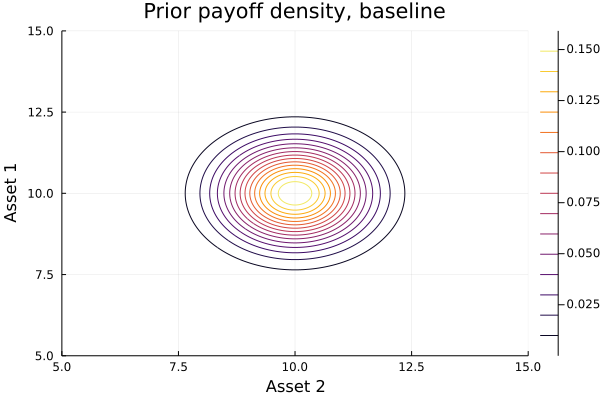
\includegraphics[width=\textwidth]{../plots/economy/baseline/prior.png}
        \end{subfigure}
    \begin{subfigure}{0.4\textwidth}
        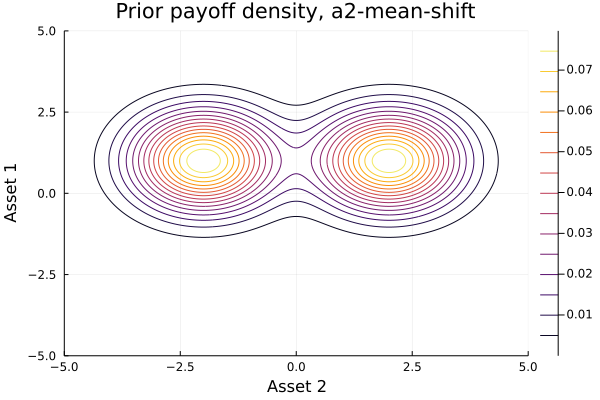
\includegraphics[width=\textwidth]{../plots/economy/a2-mean-shift/prior.png}
    \end{subfigure}
    \begin{subfigure}{0.4\textwidth}
        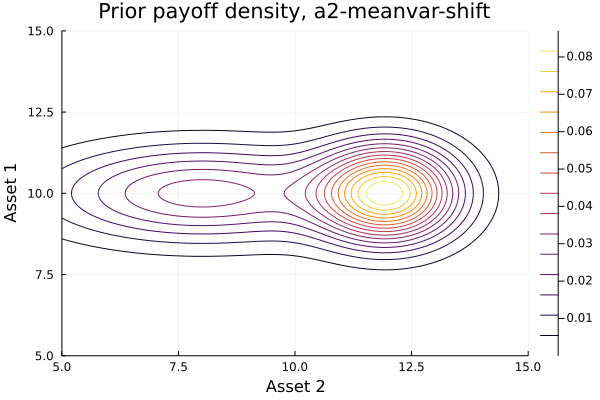
\includegraphics[width=\textwidth]{../plots/economy/a2-meanvar-shift/prior.png}
    \end{subfigure}
    \begin{subfigure}{0.4\textwidth}
        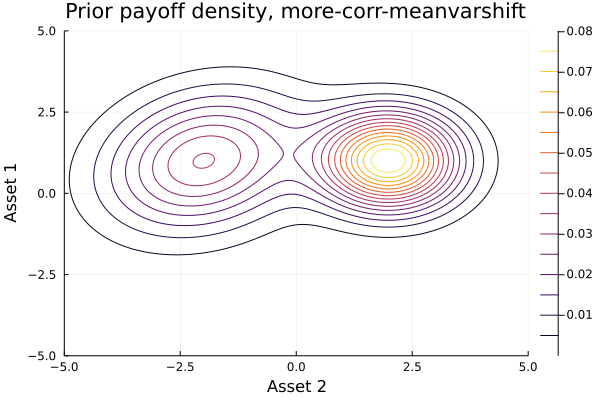
\includegraphics[width=\textwidth]{../plots/economy/more-corr-meanvarshift/prior.png}
    \end{subfigure}
    \caption{Unconditional joint payoff densities of $f$ in different economies.}
    \label{fig:priors}
\end{figure}

At present, I am most interested in how different attention allocation impacts investor beliefs and asset prices. I fix attention allocation and observe the time-2 portfolio construction problem faced by investors. Later sections will allow agents to optimize their information choices. I generate $J$ agents, half of which allocate 90\% of their attention to the safer asset 1, and the other half allocates 90\% of their attention to the riskier asset 2. Next, I assign each agent a private signal $\eta_j$ based on their attention allocation. I fix the stochastic supply to its average ($x = \bar x$) to more precisely observe equilibrium conditions.

Prices are determined through numerical minimization of the squared difference of the economy from market clearing. Denote the total quantity demanded by investors at price $p$ as $\mathbf{q}(p) = q_1(p) + q_2(p) + \dots q_J(p)$.

\begin{mini}
    {A,B,C}{\big(\mathbf{q}(p) - x\big)'\big(\mathbf{q}(p) - x\big)}
    {\label{eq:numerical-opt}}{}
    \addConstraint{p}{= A + B f + C x}
\end{mini}

The optimizer will conjecture price parameters $A$, $B$, and $C$, and then calculate all investor's posterior beliefs about the means, variances, and state probabilities conditional on the particular draw of price parameters. If the price parameters are such that net quantities $\mathbf{q}(p) - x$ is highly positive or negative, the conjectured price function cannot be the market clearing price as there exists some assets which are not held by anyone. I use the \todo{Find cite for LBFGS}LBFGS algorithm with automatic differentiation for the gradient\footnote{It has historically been more common to use finite difference gradients, but advances in computation have enabled the faster and more accurate automatic differentiation. \hl{cite Chris' paper?}}. Typically, the numerical approach yields a squared quantity disjoint around $1e^{-22}$, which is approximately exact for most numerical purposes.

\appendix
\pagebreak

\section{Figures}

\begin{figure}
    \centering
    \begin{subfigure}{0.4\textwidth}
        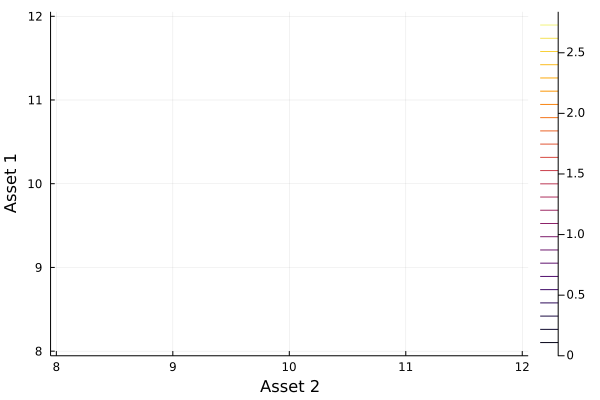
\includegraphics[width=\textwidth]{../plots/params/baseline/entropy_lower.png}
        \end{subfigure}
    \begin{subfigure}{0.4\textwidth}
        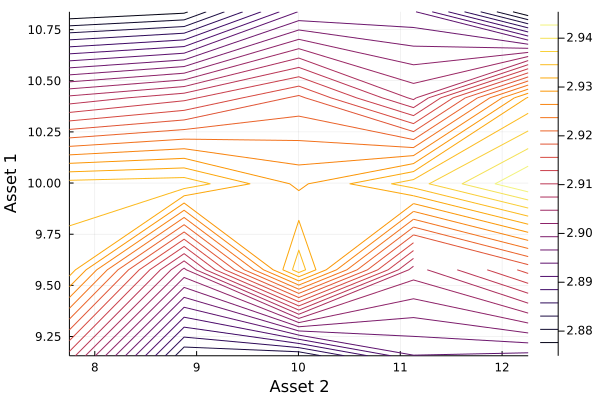
\includegraphics[width=\textwidth]{../plots/params/a2-mean-shift/entropy_lower.png}
    \end{subfigure}
    \begin{subfigure}{0.4\textwidth}
        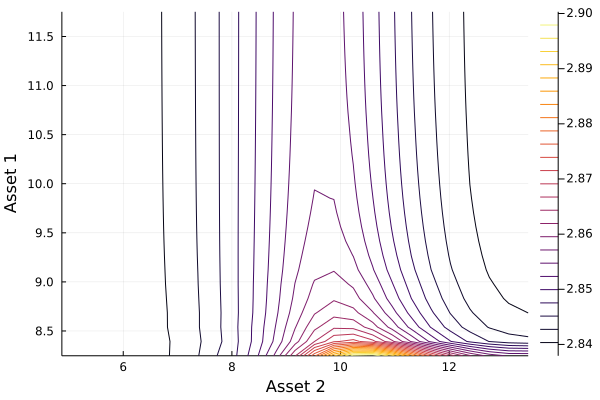
\includegraphics[width=\textwidth]{../plots/params/a2-meanvar-shift/entropy_lower.png}
    \end{subfigure}
    \begin{subfigure}{0.4\textwidth}
        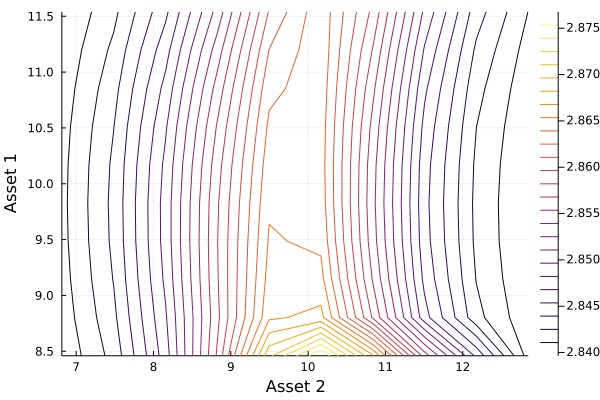
\includegraphics[width=\textwidth]{../plots/params/more-corr-meanvarshift/entropy_lower.png}
    \end{subfigure}
    \caption{Distributions of the lower bound on posterior entropy for different observations of $f$.}
    \label{fig:entropy_lower}
\end{figure}

\begin{figure}
    \centering
    \begin{subfigure}{0.4\textwidth}
        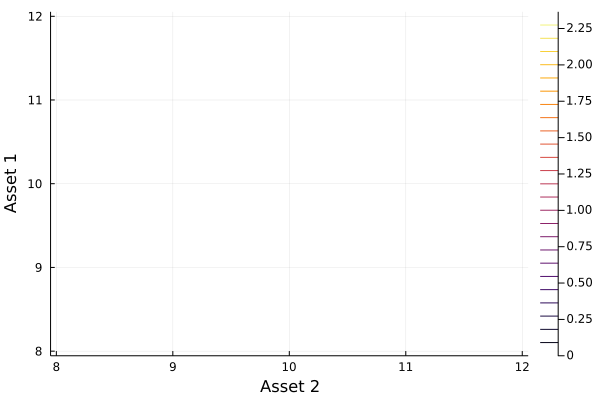
\includegraphics[width=\textwidth]{../plots/params/baseline/entropy_upper.png}
        \end{subfigure}
    \begin{subfigure}{0.4\textwidth}
        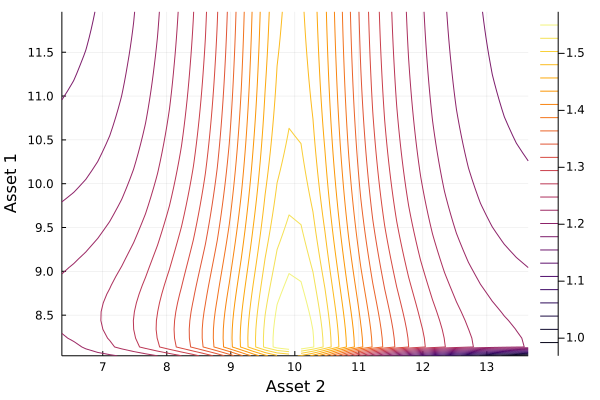
\includegraphics[width=\textwidth]{../plots/params/a2-mean-shift/entropy_upper.png}
    \end{subfigure}
    \begin{subfigure}{0.4\textwidth}
        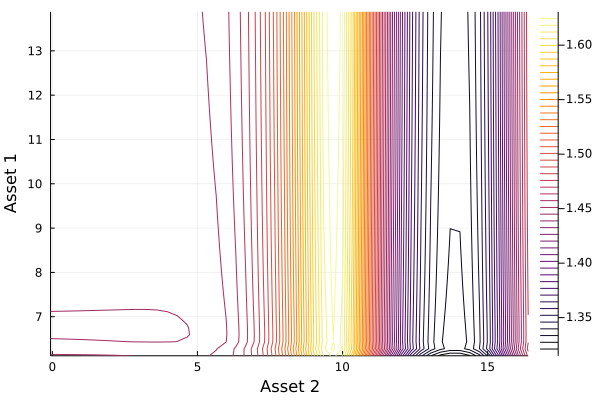
\includegraphics[width=\textwidth]{../plots/params/a2-meanvar-shift/entropy_upper.png}
    \end{subfigure}
    \begin{subfigure}{0.4\textwidth}
        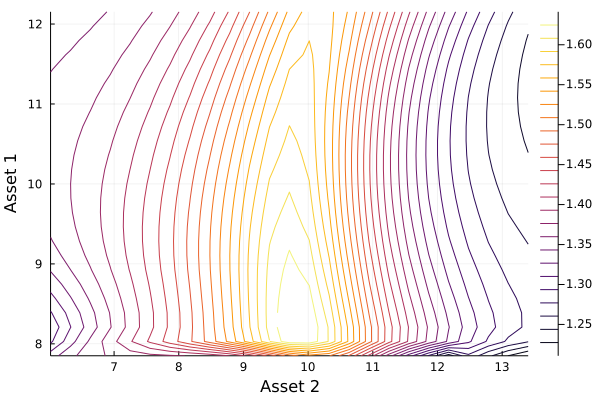
\includegraphics[width=\textwidth]{../plots/params/more-corr-meanvarshift/entropy_upper.png}
    \end{subfigure}
    \caption{Distributions of the upper bound on posterior entropy for different observations of $f$.}
    \label{fig:entropy_upper}
\end{figure}


\begin{figure}
    \centering
    \begin{subfigure}{0.4\textwidth}
        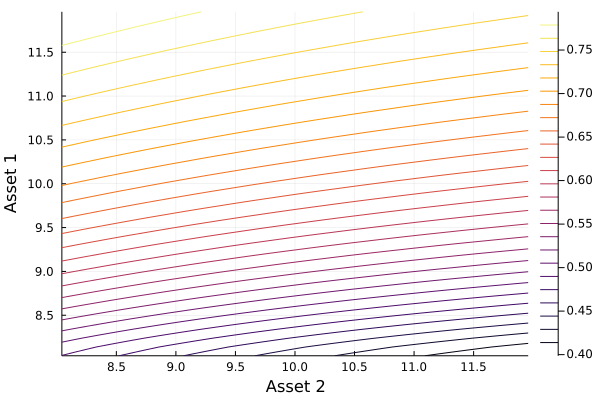
\includegraphics[width=\textwidth]{../plots/params/baseline/b11.png}
        \end{subfigure}
    \begin{subfigure}{0.4\textwidth}
        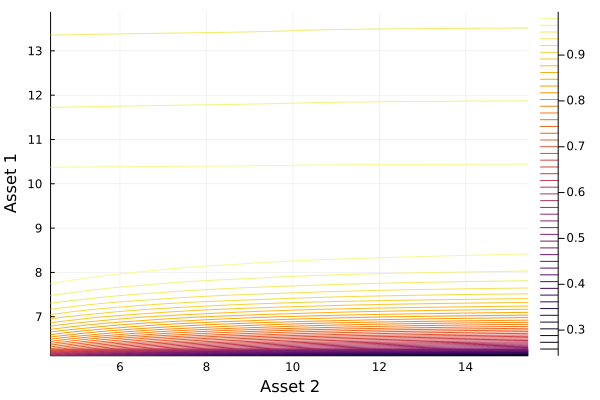
\includegraphics[width=\textwidth]{../plots/params/a2-mean-shift/b11.png}
    \end{subfigure}
    \begin{subfigure}{0.4\textwidth}
        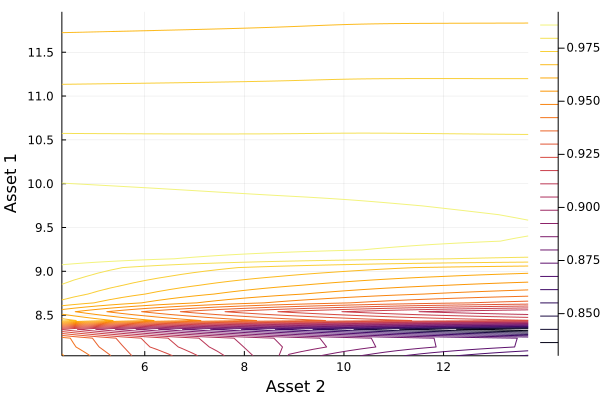
\includegraphics[width=\textwidth]{../plots/params/a2-meanvar-shift/b11.png}
    \end{subfigure}
    \begin{subfigure}{0.4\textwidth}
        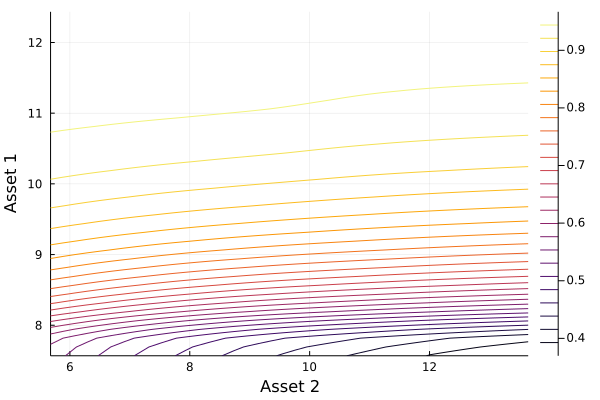
\includegraphics[width=\textwidth]{../plots/params/more-corr-meanvarshift/b11.png}
    \end{subfigure}
    \caption{Distributions of payoff coefficient matrix $B_{1,1}$ for different observations of $f$.}
    \label{fig:b11}
\end{figure}

\begin{figure}
    \centering
    \begin{subfigure}{0.4\textwidth}
        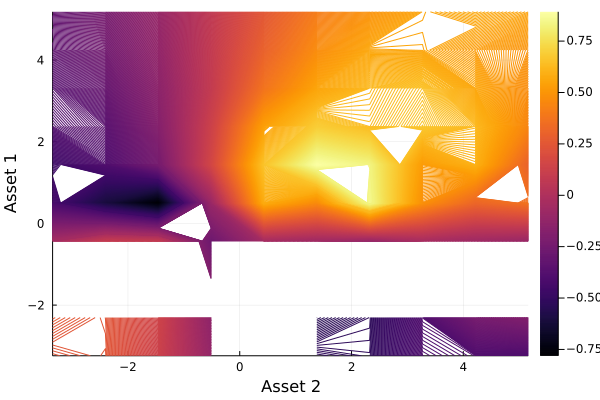
\includegraphics[width=\textwidth]{../plots/params/baseline/b22.png}
        \end{subfigure}
    \begin{subfigure}{0.4\textwidth}
        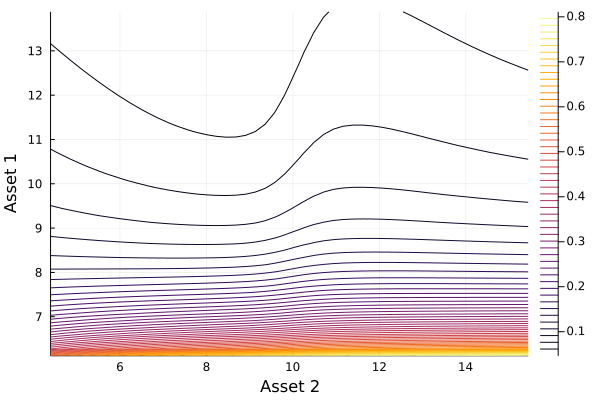
\includegraphics[width=\textwidth]{../plots/params/a2-mean-shift/b22.png}
    \end{subfigure}
    \begin{subfigure}{0.4\textwidth}
        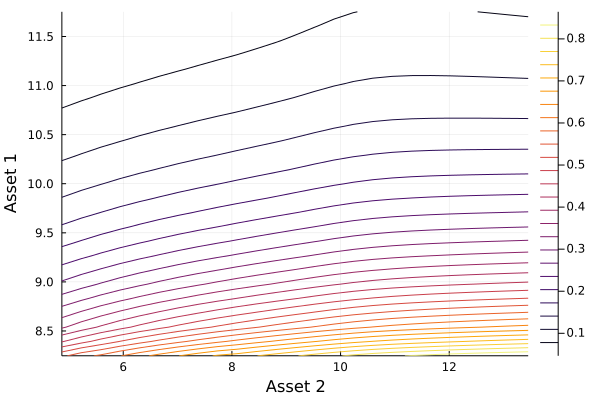
\includegraphics[width=\textwidth]{../plots/params/a2-meanvar-shift/b22.png}
    \end{subfigure}
    \begin{subfigure}{0.4\textwidth}
        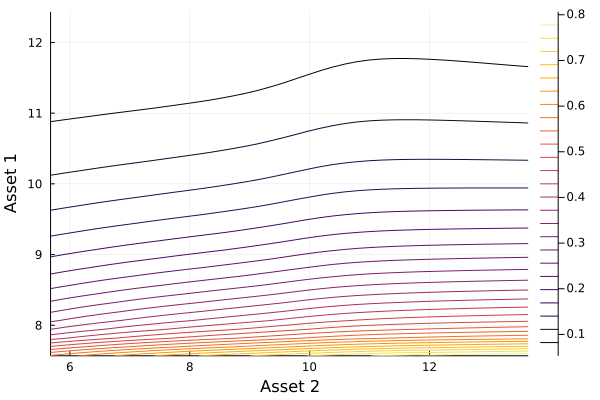
\includegraphics[width=\textwidth]{../plots/params/more-corr-meanvarshift/b22.png}
    \end{subfigure}
    \caption{Distributions of payoff coefficient matrix $B_{2,2}$ for different observations of $f$.}
    \label{fig:b22}
\end{figure}

\begin{figure}
    \centering
    \begin{subfigure}{0.4\textwidth}
        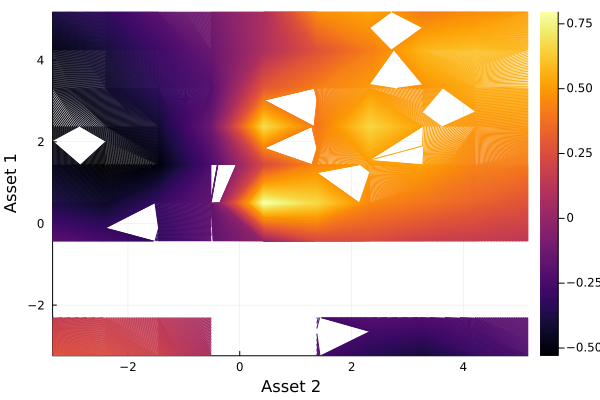
\includegraphics[width=\textwidth]{../plots/params/baseline/b12.png}
        \end{subfigure}
    \begin{subfigure}{0.4\textwidth}
        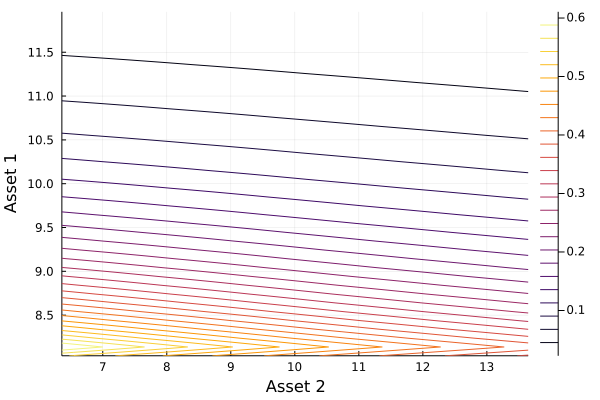
\includegraphics[width=\textwidth]{../plots/params/a2-mean-shift/b12.png}
    \end{subfigure}
    \begin{subfigure}{0.4\textwidth}
        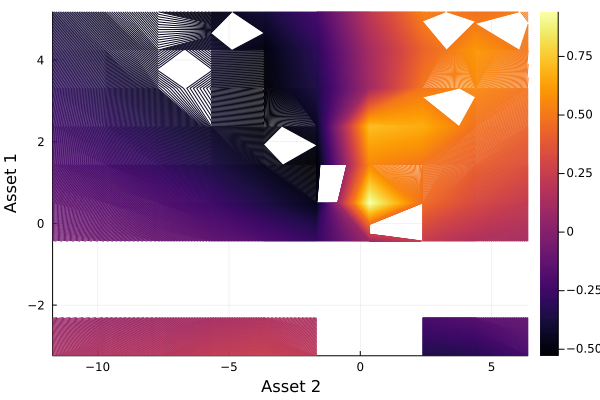
\includegraphics[width=\textwidth]{../plots/params/a2-meanvar-shift/b12.png}
    \end{subfigure}
    \begin{subfigure}{0.4\textwidth}
        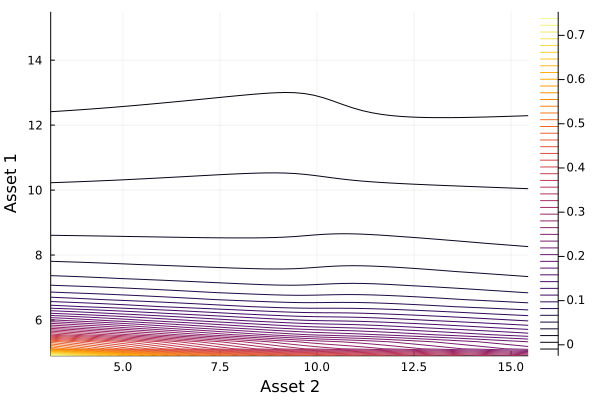
\includegraphics[width=\textwidth]{../plots/params/more-corr-meanvarshift/b12.png}
    \end{subfigure}
    \caption{Distributions of payoff coefficient matrix $B_{1,2}$ for different observations of $f$.}
    \label{fig:b12}
\end{figure}

\begin{figure}
    \centering
    \begin{subfigure}{0.4\textwidth}
        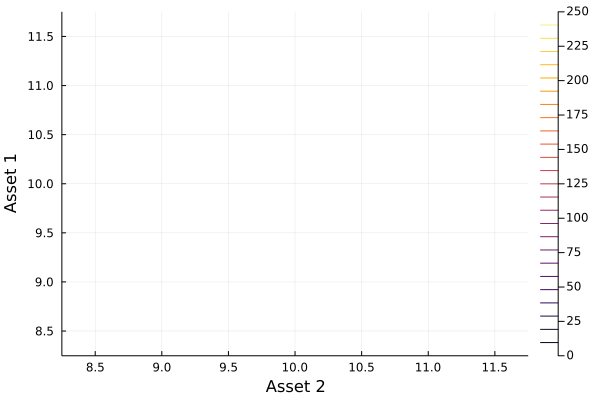
\includegraphics[width=\textwidth]{../plots/params/baseline/disagreement.png}
        \end{subfigure}
    \begin{subfigure}{0.4\textwidth}
        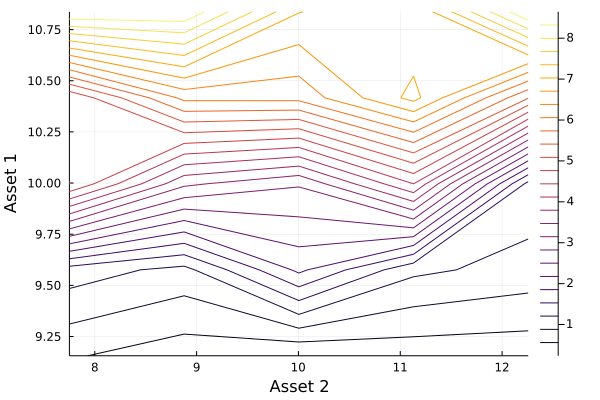
\includegraphics[width=\textwidth]{../plots/params/a2-mean-shift/disagreement.png}
    \end{subfigure}
    \begin{subfigure}{0.4\textwidth}
        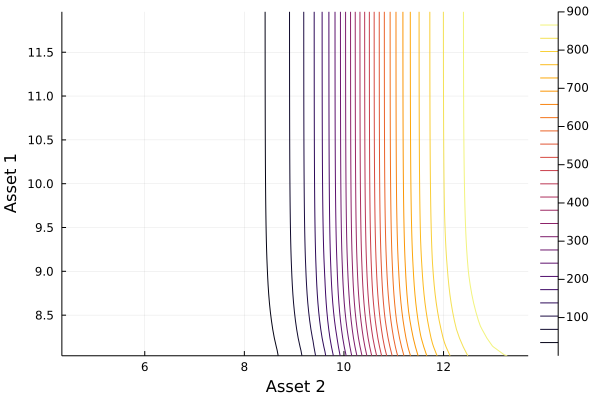
\includegraphics[width=\textwidth]{../plots/params/a2-meanvar-shift/disagreement.png}
    \end{subfigure}
    \begin{subfigure}{0.4\textwidth}
        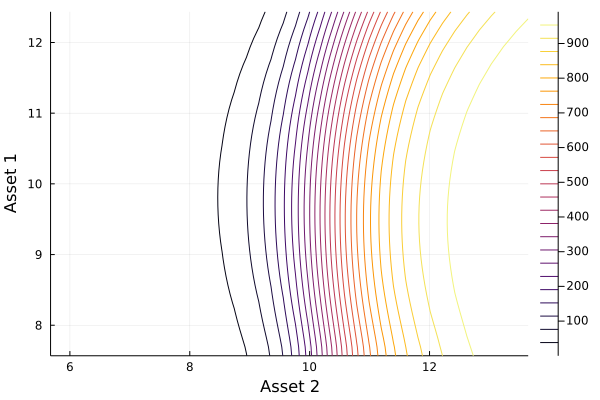
\includegraphics[width=\textwidth]{../plots/params/more-corr-meanvarshift/disagreement.png}
    \end{subfigure}
    \caption{Distributions of disagreement ($\sum \hat s_j^2$) for different observations of $f$.}
    \label{fig:disagreement}
\end{figure}

\begin{figure}
    \centering
    \begin{subfigure}{0.4\textwidth}
        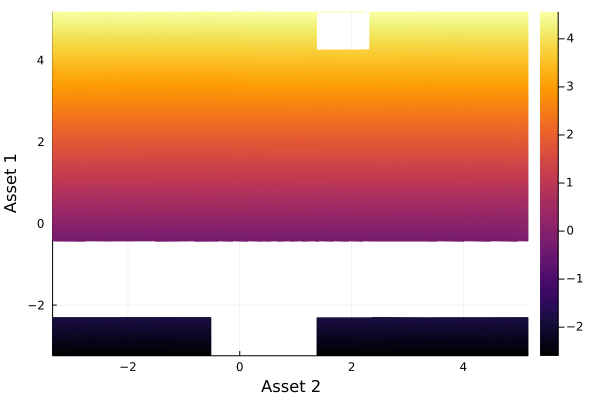
\includegraphics[width=\textwidth]{../plots/params/baseline/p1.png}
        \end{subfigure}
    \begin{subfigure}{0.4\textwidth}
        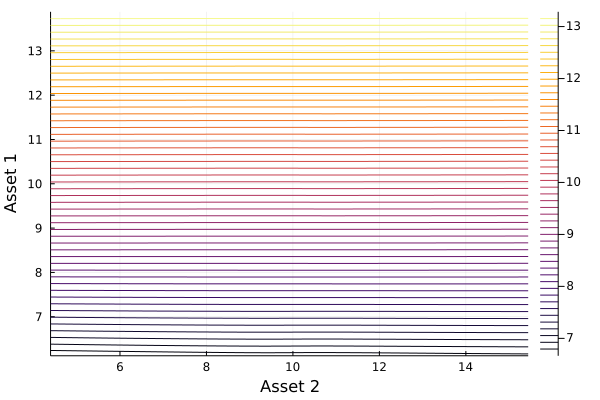
\includegraphics[width=\textwidth]{../plots/params/a2-mean-shift/p1.png}
    \end{subfigure}
    \begin{subfigure}{0.4\textwidth}
        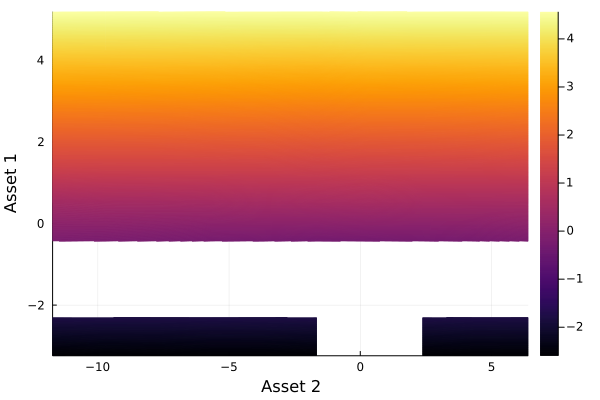
\includegraphics[width=\textwidth]{../plots/params/a2-meanvar-shift/p1.png}
    \end{subfigure}
    \begin{subfigure}{0.4\textwidth}
        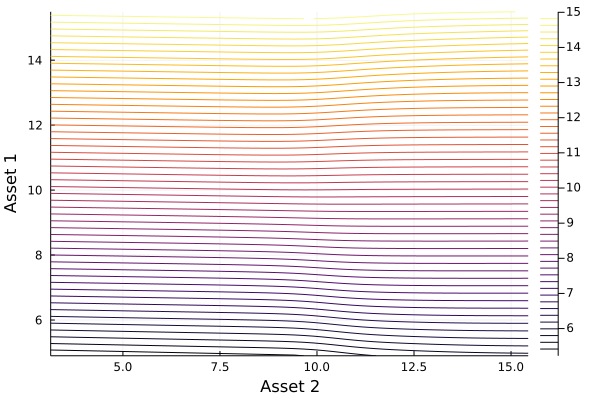
\includegraphics[width=\textwidth]{../plots/params/more-corr-meanvarshift/p1.png}
    \end{subfigure}
    \caption{Distributions of the asset 1 price for different observations of $f$.}
    \label{fig:p1}
\end{figure}

\begin{figure}
    \centering
    \begin{subfigure}{0.4\textwidth}
        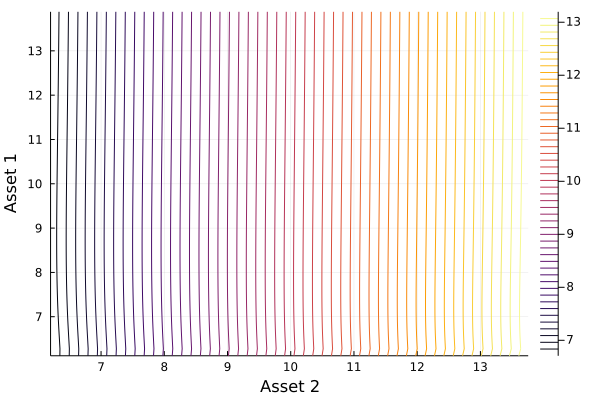
\includegraphics[width=\textwidth]{../plots/params/baseline/p2.png}
        \end{subfigure}
    \begin{subfigure}{0.4\textwidth}
        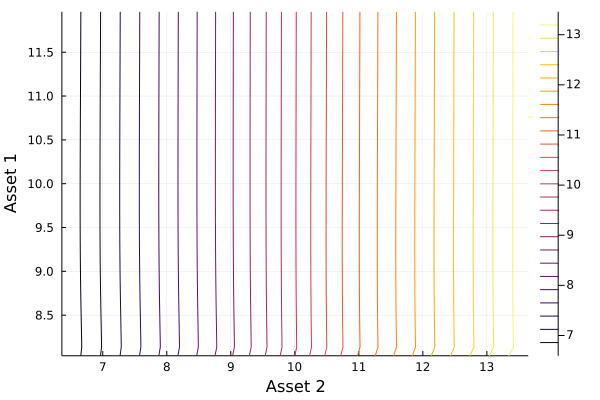
\includegraphics[width=\textwidth]{../plots/params/a2-mean-shift/p2.png}
    \end{subfigure}
    \begin{subfigure}{0.4\textwidth}
        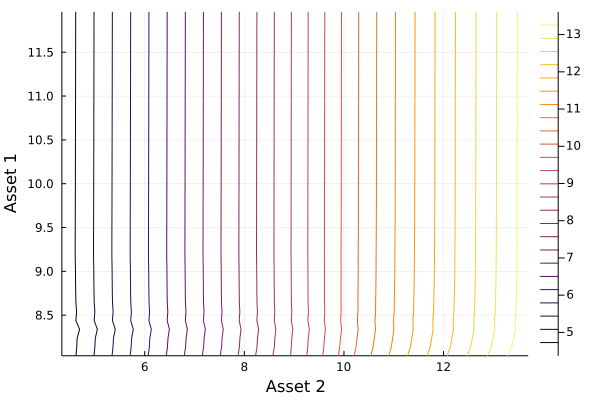
\includegraphics[width=\textwidth]{../plots/params/a2-meanvar-shift/p2.png}
    \end{subfigure}
    \begin{subfigure}{0.4\textwidth}
        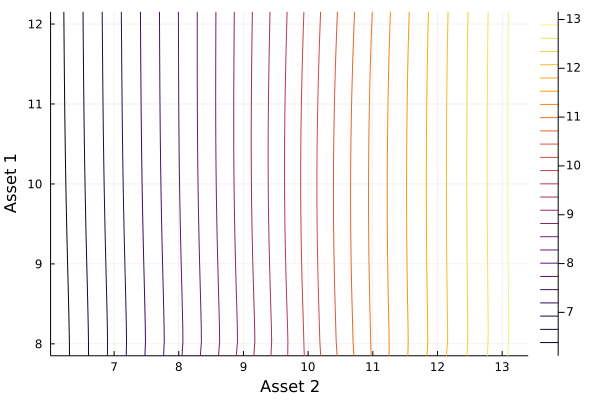
\includegraphics[width=\textwidth]{../plots/params/more-corr-meanvarshift/p2.png}
    \end{subfigure}
    \caption{Distributions of the asset 2 price for different observations of $f$.}
    \label{fig:p2}
\end{figure}



% \begin{figure}
%     \centering
%     \begin{subfigure}{0.4\textwidth}
%         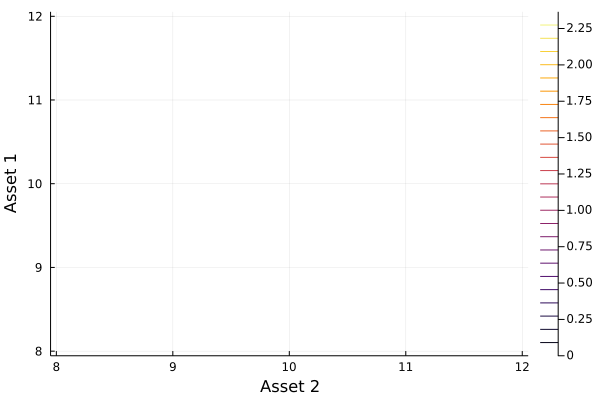
\includegraphics[width=\textwidth]{../plots/params/baseline/entropy_upper.png}
%         \end{subfigure}
%     \begin{subfigure}{0.4\textwidth}
%         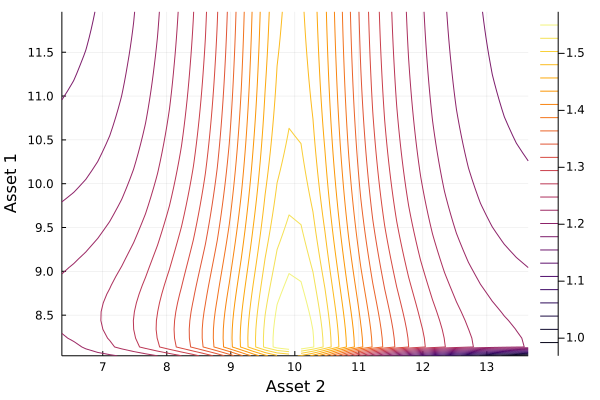
\includegraphics[width=\textwidth]{../plots/params/a2-mean-shift/entropy_upper.png}
%     \end{subfigure}
%     \begin{subfigure}{0.4\textwidth}
%         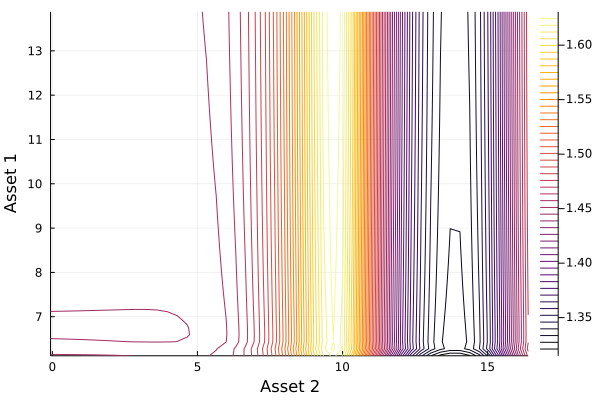
\includegraphics[width=\textwidth]{../plots/params/a2-meanvar-shift/entropy_upper.png}
%     \end{subfigure}
%     \begin{subfigure}{0.4\textwidth}
%         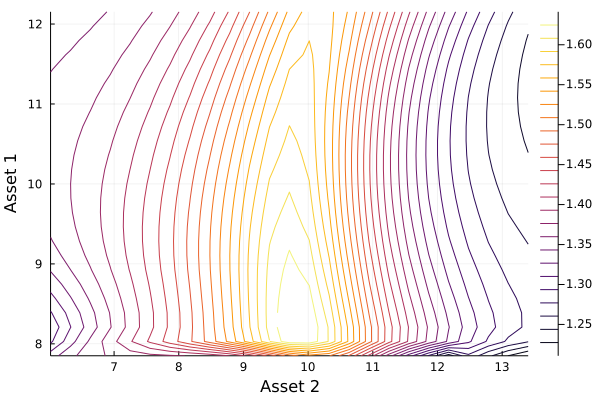
\includegraphics[width=\textwidth]{../plots/params/more-corr-meanvarshift/entropy_upper.png}
%     \end{subfigure}
%     \caption{Distributions of the upper bound on posterior entropy for different observations of $f$.}
%     \label{fig:entropy_upper}
% \end{figure}

\section{Mixture model variance}

The variance-covariance matrix of variable $X$ following a Gaussian mixture distribution with means $\mu = [\mu_1, \mu_2, \dots, \mu_k]'$, covariances $\Sigma= [\Sigma_1, \Sigma_2, \dots, \Sigma_k]$, and mixture proportions $\pi = [\pi_1, \pi_2, \dots, \pi_k]'$ is\footnote{From https://math.stackexchange.com/questions/195911/calculation-of-the-covariance-of-gaussian-mixtures} 

\begin{align}
    \Var[X] &= E[\Var[X \mid k]] + \Var[E[X \mid k]] \\
            &= \sum_k  \pi_k  \bigg(\Sigma_k + (\mu_k - \overline{\mu})(\mu_k - \overline{\mu})' \bigg)
\end{align}

\noindent for $\overline{\mu}=\sum_k \pi_k \mu_k$.

\section{Misc identities}

Stochastic variables:

\begin{itemize}
    \item State variable $s ~ \sim \text{Bernoulli}(\pi)$. $P(s=H) = \pi$, $P(s=L) = 1-\pi$.
    \item Risk factor payoffs $\tilde f \mid s \sim N(\Gamma^{-1} \mu_s, \Sigma_s)$
    \item Risk factor supply $x \sim N(\overline{x}, \sigma_x I)$
    \item Private signals $\eta_j \mid s \sim N(z, \Sigma_{\eta_j})$
    \item Price signal $\eta_p \mid s \sim N(z, \Sigma_p)$
\end{itemize}

Joint density:

$$
P(s, \tilde f, x, \eta_j, \eta_p) = P(\tilde f \mid s) P(\eta_j \mid s) P(\eta_p \mid s) P(s)  P(x)
$$

Posterior density:

$$
P(s, \tilde f \mid x, \eta_j, \eta_p) = 
    \frac{
        P(x, \eta_j, \eta_p \mid s, \tilde f) P(s, \tilde f)
    }{
        P(x, \eta_j, \eta_p)
    }
$$

Unknown values:

\begin{itemize}
    \item $E_j[\tilde f - \tilde p r \mid H]$
    \item $E_j[\tilde f - \tilde p r \mid L]$
    \item $V_j[\tilde f - \tilde p r \mid H]$
    \item $V_j[\tilde f - \tilde p r \mid L]$
    \item $P(H \mid \eta_p, \eta_j)$
    \item $P(L \mid \eta_p, \eta_j)$
    \item $E_j[\tilde f \mid \eta_p, \eta_j]$
    \item $V_j[\tilde f \mid \eta_p, \eta_j]$
    \item $\tilde p$
\end{itemize}

Portfolio choice problem:

\begin{align*}
    U_{2j} &= \max_{\tilde q_j}
        \rho E_j [W_j] - \frac{\rho^2}{2} V_j [W_j] \\
\end{align*}

Optimal quantity:

\begin{align*}
    \tilde q_j &= \frac1\rho \bigg( P(H) \Sigma_H + P(L) \Sigma_L \bigg)^{-1} \bigg(
        P(H) E_j [\tilde f \mid H] + P(L) E_j [\tilde f \mid L] - \tilde p r
    \bigg) \\
    &= \frac1\rho V_j[\tilde f]^{-1} (E_j [\tilde f] - \tilde p r)
\end{align*}

Ex-ante expected utility:

\begin{align*}
    U_{1j} &= E\biggl[
        \rho E_j [W_j] - \frac{\rho^2}{2} V_j [W_j]
    \biggr] \\
    &= 
        \pi E\biggl[
            \rho E_j [W_j \mid H] - \frac{\rho^2}{2} V_j [W_j \mid H]
        \biggr] \\
        &\quad +
        (1-\pi) E\biggl[
            \rho E_j [W_j \mid L] - \frac{\rho^2}{2} V_j [W_j \mid L]
        \biggr] \\
    &= \rho r W_0 \\
        &\quad + 
        \rho \tilde q'_j \biggl(
            \pi E_j [\tilde f - \tilde p r \mid H] +
            (1-\pi) E_j [\tilde f - \tilde p r \mid L]
        \biggr) \\
        &\quad -
        \frac{\rho^2}{2} \tilde q'_j \biggl(
            \pi V_j [\tilde f - \tilde p r \mid H] +
            (1-\pi) V_j [\tilde f - \tilde p r \mid L]
        \biggr) \tilde q_j
\end{align*}


% \newpage
% \printbibliography

\end{document}
